\documentclass[12pt]{report}
% \documentclass[12pt, draft]{report}
\usepackage{ifdraft} % used for draft visualization
\usepackage[english]{babel}
\usepackage{setspace}
\usepackage{graphicx}
\usepackage{xcolor}
\usepackage{mathtools}
\usepackage{mathdots}
\usepackage{braket}
\usepackage{cancel}
\usepackage{amsmath}
\usepackage{amssymb}
\usepackage{amsfonts}
\usepackage{siunitx}
\usepackage{enumitem}
\usepackage{bm} % used for /bm -> bold math
\usepackage{comment}
\usepackage{float}
\usepackage{nicefrac, xfrac}
\usepackage{caption}
\usepackage{array}

% graphs packages
\usepackage{tikz}
% \usepackage{pgfplots}

\usepackage{listings,lstautogobble} % il secondo aggiusta l'indentazione del codice
\lstset{
    autogobble=true,
    aboveskip=10pt,
    belowskip=10pt,
}
\usepackage{matlab-prettifier} % used for pretty matlab snippets
\begin{comment}
    \begin{lstlisting}
    [style=Matlab-editor, numbers=left, columns=fullflexible, escapechar=\#]
    \end{lstlisting}
\end{comment}

\begin{comment}
    MATLAB color palette
    gem = [
   "#0072bd"; % dark blue
   "#d95319"; % dark orange
   "#edb120"; % dark yellow
   "#7e2f8e"; % dark magenta
   "#77ac30"; % dark green
   "#4dbeee"; % dark blue sky
   "#a2142f"; % dark red blood
   "#ffd60a"; % sunflower yellow
   "#6582fd"; % discord violet
   "#ff453a"; % watermelon red
   "#1fcfbe"; % acquamarina
   "#268cdd"; % light blue
];
\end{comment}

\usepackage{titlesec}
% impostazioni per i titoli
\titleformat{\chapter}[display]
{\normalfont\LARGE\bfseries} % stile e dimensione del testo "Chapter X"
{\chaptertitlename\ \thechapter}
{20pt} % spazio tra il numero del capitolo ed il testo
{\Huge} % dimensione del testo del capitolo

% impostazione per l'header (e lo stile in generale) della pagina
\newpagestyle{main}{
    \headrule
    \sethead[][][\textsc{\sectiontitle}]
            {}{}{\textsc{\sectiontitle}}
    \setfoot{}{\thepage}{}
}
\pagestyle{main}

\usepackage[parfill]{parskip} % toglie l'indentazione della prima riga dopo un nuovo paragrafo

\usepackage{perpage} % pacchetto per gestore i footnotes
\usepackage[bottom, hang, flushmargin]{footmisc} % inserisce i footnotes al fondo della pagina
% resetta il counter dei footnotes ad ogni sezione
\makeatletter
\@addtoreset{footnote}{section}
\makeatother
% \MakePerPage{footnote} % resetta il counter dei footnotes ad ogni pagina

\usepackage{caption}
% imposta la spaziatura tra le figure e quello che viene prima e dopo
\setlength{\floatsep}{15pt} % spazio tra figure
\setlength{\textfloatsep}{15pt} % spazio tra il testo e la figura
\setlength{\intextsep}{15pt} % spazio per le figure in-text
\setlength{\belowcaptionskip}{15pt} % spazio dopo la caption

\begin{document}
    \onehalfspacing

    % imposta la spaziatura tra testo ed equazioni metematiche
    \abovedisplayskip = 10.5pt
    \abovedisplayshortskip = 10.5pt
    \belowdisplayskip = 10.5pt
    \belowdisplayshortskip = 10.5pt

    \setitemize{labelindent=1.5em, labelsep=15pt, leftmargin=*} % impostazioni per le bullet-list (usa il pacchetto enumitem)

    \setlength{\jot}{12pt} % spaziature negli enviroment multilinea "gather" o in generale di asmmath

    % -----------------------------------
    \begin{titlepage}
        \vspace*{\fill}
        \begin{center}
            \LARGE
            \textbf{\uppercase{weather to walk or\\run in the rain}}\\
            \vspace{30pt}
            \Large
            A numerical approach to a \\practical problem\\
        \end{center}
        \vspace{300pt}
        \begin{center}
            \large
            \textbf{Simone Albano}\\
            December, 2024
        \end{center}
        \vspace*{\fill}
    \end{titlepage}
    % -----------------------------------

    % inizio del documento effettivo
    \newpage
    \pagenumbering{arabic}

    \chapter{Method introduction}
    The question we aim to address in this short document is whether it is better to walk or run when caught in the rain. Conducting real tests with actual rain would be both impractical and time-consuming, so we will attempt to answer this question through numerical simulations.

    We will also explore whether factors such as the horizontal speed and angle of the rain significantly impact the outcome. Additionally, we will investigate whether varying the proportions of the object used to simulate the human body can help minimize exposure to raindrops.

        \newpage
        \section{Rain generation algorithm}
            We will start our investigation by creating a virtual rainy environment using the MATLAB software. The \underline{simulation box} is defined as the rectangular domain within which all raindrops are considered "active." This means we will only count the raindrops that hit the object emulating the human body when it is inside the simulation box. This approach is necessary because, when the angle of the rain with respect to the floor normal is set to a value other than zero, we must ensure that the entire path from the starting point to the ending point is covered by rain.

            The algorithm for generating the rain is very simple: at each discrete time step $t_k$, a new vector of raindrops of length $N$ is generated. This vector is a horizontal, uniformly spaced array containing the $x$ and $y$ coordinates of the $N$ generated drops, positioned at the highest $y$ coordinate of the simulation box. For the reason explained earlier, raindrops are also generated outside the horizontal bounds of the simulation box. To create a more realistic setup, a zero-mean Gaussian noise vector of length $N$ is added to the coordinates of the newly generated raindrops. (Using a zero-mean normal noise distribution is essential to maintain a constant rain density, as deviations could introduce unwanted biases into the results.)
            
            In the same iteration of the algorithm, we update the position of the raindrop vector generated at step $t_{k-1}$ according to the rain velocity parameter $V_r$. Since it is crucial to maintain a constant vertical component of the rain velocity to ensure consistent rain density across all simulations, we will treat this parameter as a global constant. 
            
            \newpage
            The horizontal velocity of the rain will then be calculated using the rain angle $\vartheta_r$ with the following relation:
            \begin{equation}
            V^{rain}_x = \frac{V^{rain}_y}{\tan(\vartheta_r - \frac{\pi}{2})}
            \end{equation}
            In order to avoid to overload the algorithm with an absurd amount of rain drops, we will destroy all the drops that exit the bottom floor of the simulation box, since they are no longher needed. Furthermore, we will also remove all the drops that hits the target object since in a real life situation these drops are going to be absorbed by the person clothes.

            The part of the algorithm that detects the collisions with the object under test is again very rudimental: we can simply detect a collision by looking at the coordinates of the rain drop, and compare them to the position of the rectangle emulating the body. If the drop is located inside the rectangle, a collision is detected, and the counter holding the total number of hits is incremented. Since the rain speed is going to be limited with respect to the simulation speed, we are going to avoid the checks for tunneling collisions (a type of collision where the drop bypasses completely the target due to very high speeds).

            Another very important factor that our algorithm needs to take into account is the size of the rectangle used to mimic the human body: in order to make the simulation as realistic as possible, we are going to use an heigth-to-thickness ratio of six, that is valid for the vast majority of people. We will later observe that the amount of rain that falls on our head cannot be optimized, and thus removed. Another round of simulations will be carried out by changing the proportions of our rectangle in order to emulate the behaviour of a cat (whose body heigth-to-thickness proportion is one-third). 
            
            \newpage
            The following figure shows one of the many performed simulations:
            \begin{figure}[H]
                \centering
                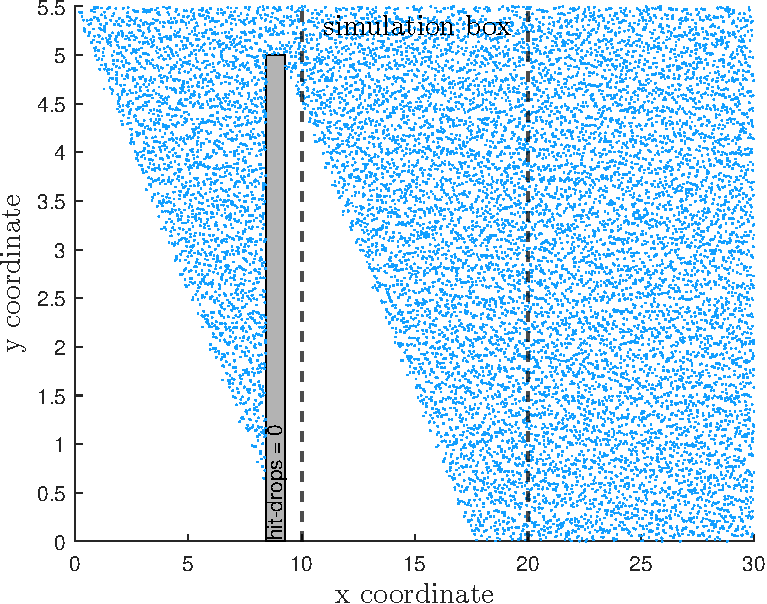
\includegraphics[width=0.9\textwidth]{images/sim.pdf}
                \caption{An example of a simulation with a rain angle $\vartheta_r = \frac{\pi}{3}$: the count begins only when the object enters the simulation box. In general, a positive rain angle $\vartheta_r$ indicates that the rain is falling behind the test subject, whereas a negative rain angle means the rain is coming from the opposite direction relative to the test object's movement.}
            \end{figure}
            \vspace{-30pt}
            Here are reported the parameters used for all the simulations:
            \begin{itemize}
                \item The simulation box is the rectangle $[10, 20] \times [0, 5.5]$.
                \item The rain is generated at $y = 5.5$ in the interval $x \in [0, 30]$.
                \item Every rain drops vector contains a number of drops equal to $N = 512$.
                \item The global rain vertical velocity is equal to $V^{rain}_y = -0.150$ m/s.
                \item The body rectangle has dimensions $L = 0.83m, \text{ } H = 5m$.
            \end{itemize}

            \newpage
        \section{Results obtained for the human body}
            A total of 4096 different simulations were performed by varying the rain angle and object speed within the ranges $\vartheta_r \in [-\frac{\pi}{3}, \frac{\pi}{3}]$ and $V^{obj}_x \in [0.005, 0.3]$ m/s, discretized into 64 steps each. The following plots present the obtained results.
            \begin{figure}[H]
                \centering
                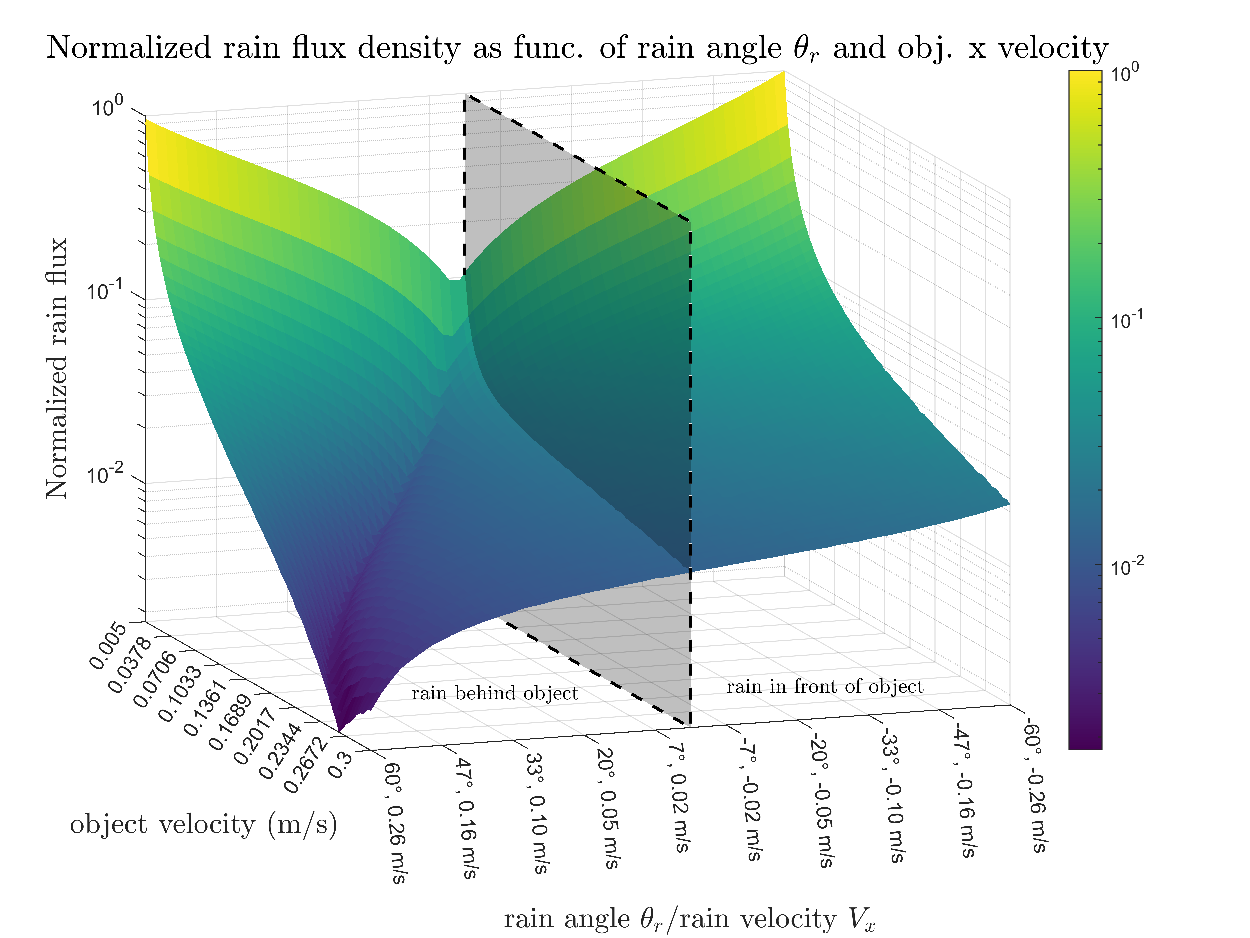
\includegraphics[width=1\textwidth]{images/human/rain_flux_surf_3D.pdf}
                \caption{Here is reported the full 3D view of the function that shows the normalized rain flux density that hits the target body as a function of both the rain angle $\vartheta_r$ and body velocity $V^{obj}_x$.}
            \end{figure}
            \vspace{-30pt}
            To our surprise, we can clearly observe that for positive values of the rain angle $\vartheta_r$, there are points where the amount of rain hitting the test rectangle decreases significantly. To investigate further, we should examine some cross-sections of the surface.

            \newpage
            \begin{figure}[H]
                \centering
                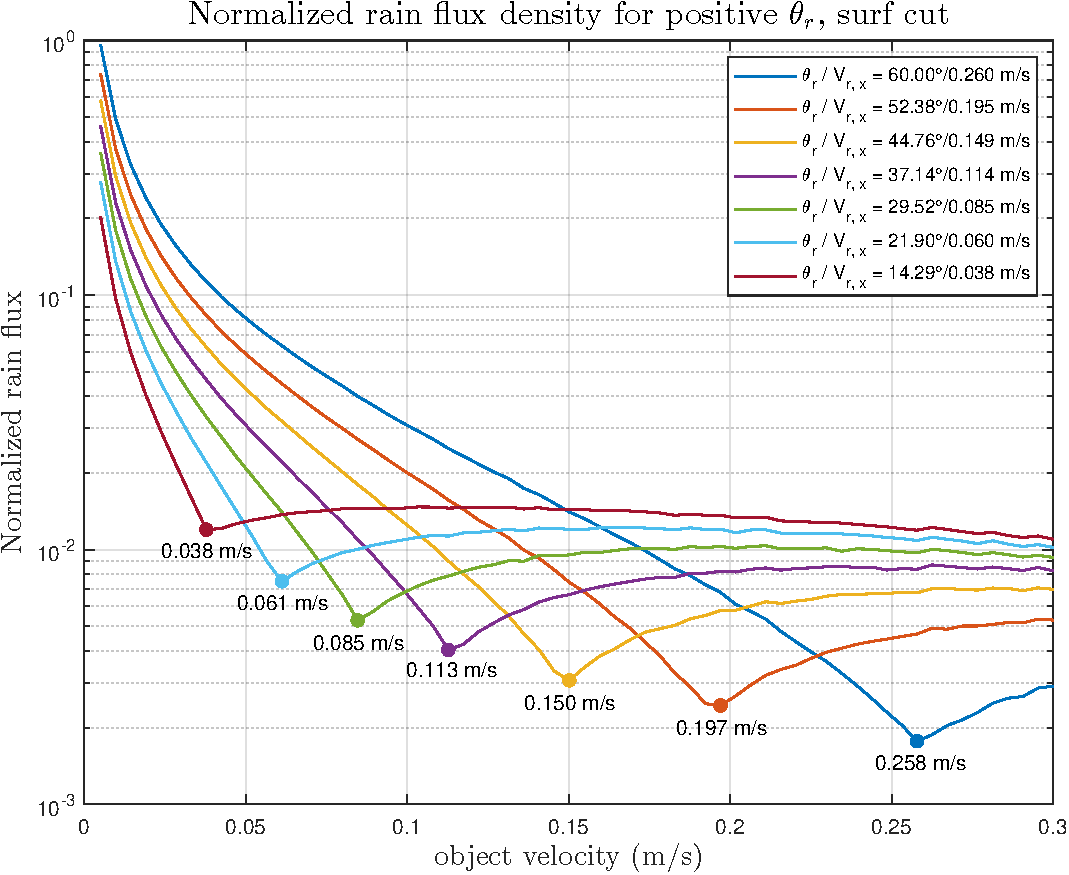
\includegraphics[width=0.9\textwidth]{images/human/rain_flux_vx_min.pdf}
                \caption{2D cut performed along the zy plane. The different curves represent the rain fluxes for different rain angles.}
            \end{figure}
            \vspace{-30pt}
            The results speak for themselves: the curves representing the rain flux densities as a function of the test object's speed for different positive values of the rain angle $\vartheta_r$ show that the rain exposure can be minimized by traveling with a speed equal to the horizontal component of the raindrop velocity. This can be interpreted as follows: by running at a speed that matches the horizontal component of the rain's velocity, we are essentially "escaping" the raindrops that are trying to reach our back. If our velocity does not match the rain's horizontal speed, we will be hitted by raindrops either behind or in front of us, depending on whether we are traveling slower or faster than the optimal speed. Additionally, we can observe that traveling faster than the optimal speed does not reduce significantly the number of hitted drops.

            \newpage
        \section{Results obtained for the cat-shaped body}
            The same simulations are performed again using a test rectangle that resembles the proportions of a cat. The idea is that, since the raindrops falling vertically onto the test subject cannot be optimized, the cat-shaped object will exhibit a reduced dependence of rain flux density on its horizontal speed under the rain.
            \begin{figure}[H]
                \centering
                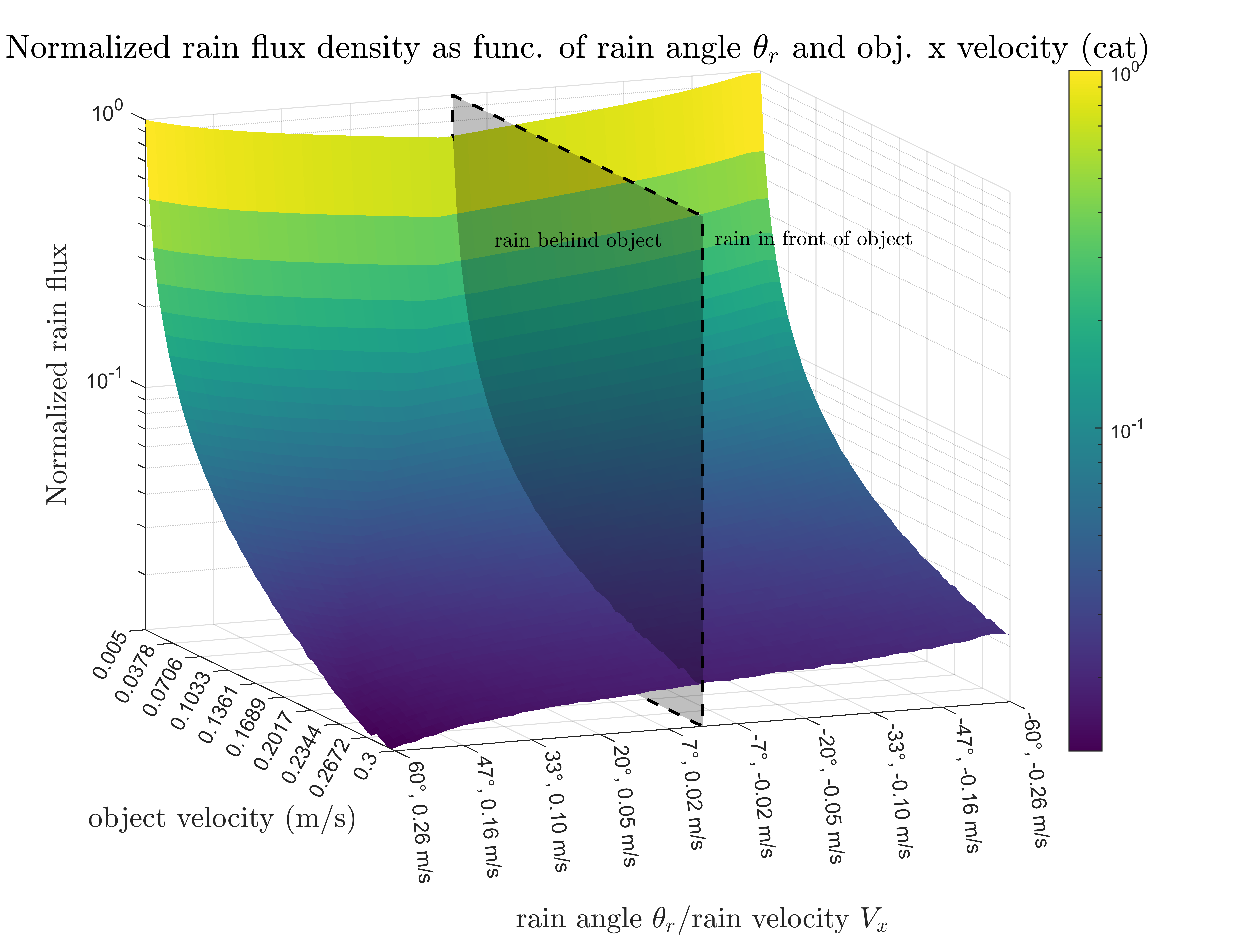
\includegraphics[width=1\textwidth]{images/cat/rain_flux_surf_3D_cat.pdf}
                \caption{Full 3D surface of the rain flux density in the case of the cat as a function of both the rain angle $\vartheta_r$ and body velocity $V^{obj}_x$.}
            \end{figure}
            \vspace{-30pt}
            As predicted earlier, the dependence of the rain flux from the cat horizontal speed is practically absent.

            \newpage
            This is confermed even if we take a look at the same cut of the surface performed in the case of the human body.
            \begin{figure}[H]
                \centering
                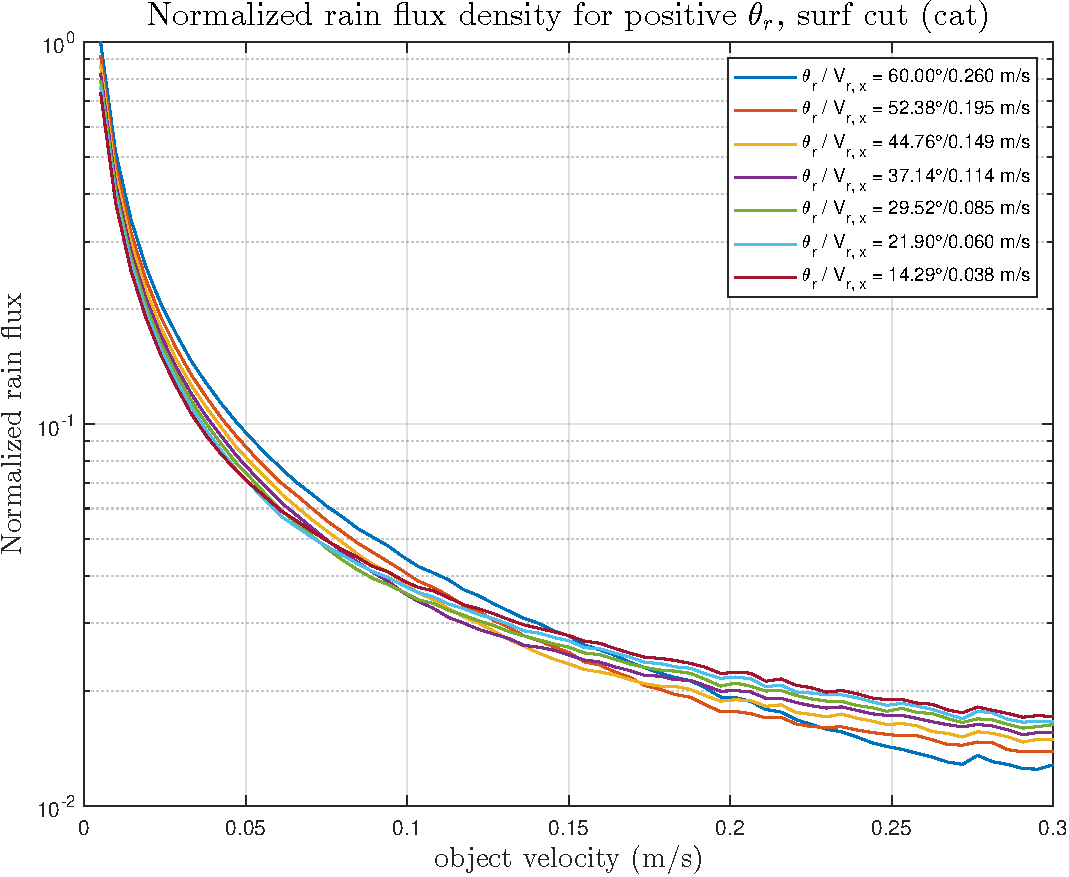
\includegraphics[width=0.9\textwidth]{images/cat/rain_flux_vx_min_cat.pdf}
                \caption{2D cut performed along the zy plane where the different curves represent the rain fluxes for different rain angles. The absence of any points of minima conferms our theory.}
            \end{figure}
            \vspace{-30pt}
            This behavior can be explained by the fact that the only surfaces contributing to the dependence of rain flux density on the cat's speed are the front and back sides of the rectangle emulating the cat. These surfaces are relatively small compared to the top surface, which is always exposed to the rain.

            \newpage
        \section{Conclusions}
            In this study, we examined the effect of walking versus running in the rain through numerical simulations. By varying the rain angle and the horizontal speed of the test object, we found that there is an optimal speed equal to the horizontal component of the rain's velocity that minimizes the amount of rain hitting the test subject. This result can be interpreted as "escaping" the rain by matching the rain's horizontal speed.

            Furthermore, when using a cat-shaped object, we observed a reduced dependence of rain flux density on horizontal speed. This is due to the smaller front and back surfaces of the object compared to the top surface, which remains exposed to the rain. Overall, the study shows that while increasing speed beyond the optimal value yields minimal additional benefit, adjusting speed to match the horizontal component of the rain can significantly reduce exposure.

            For negative values of the rain angle, the best strategy is always to run, as running faster helps reduce the rain flux through the body. Increasing speed in these cases leads to a greater reduction in exposure to raindrops.

            In the following pages additional plots and figures that has been produced during the simulation process can be found.

            \newpage
            Additional figures for the case of the simulation of the human body:
            \vspace{-10pt}
            \begin{figure}[H]
                \centering
                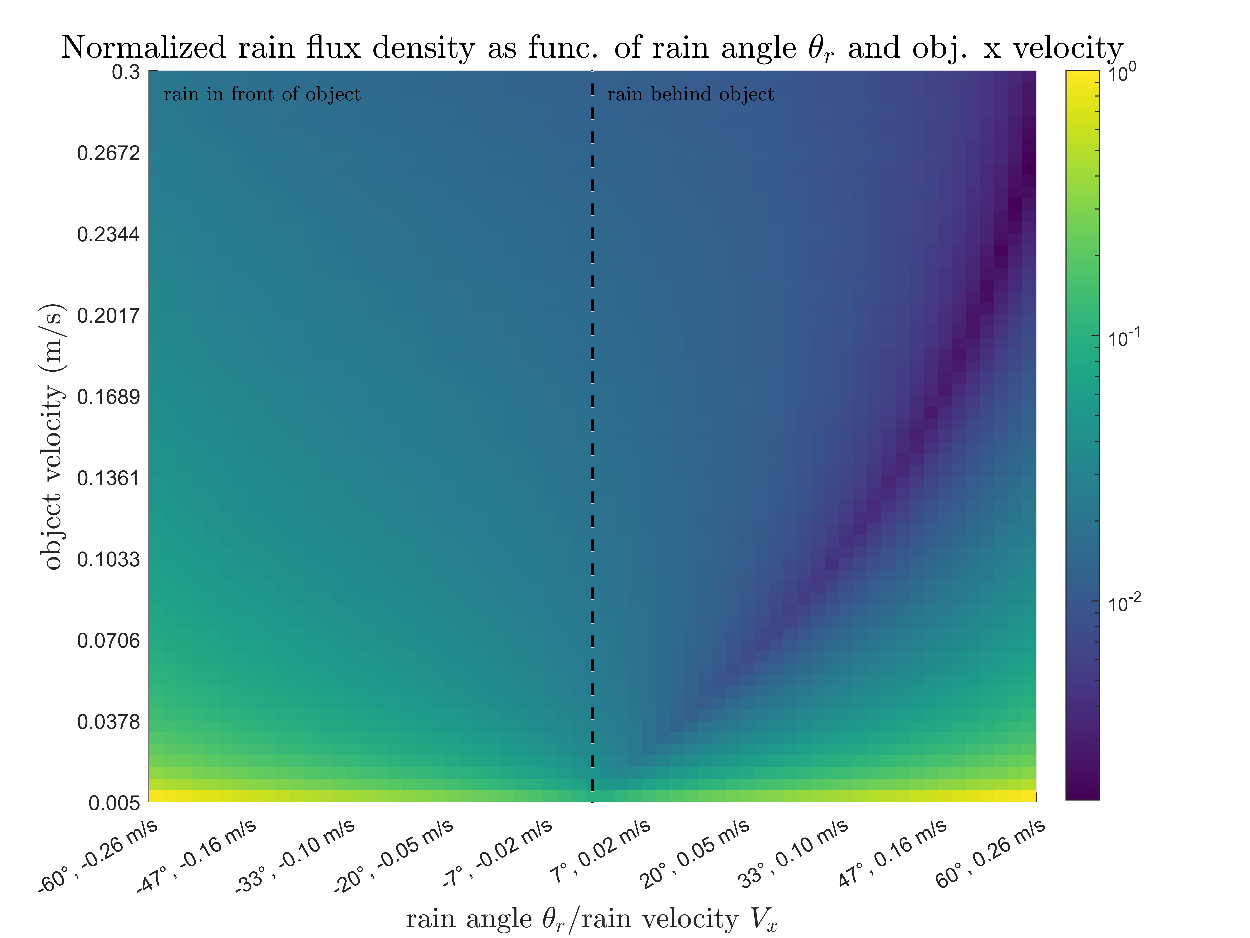
\includegraphics[width=0.725\textwidth]{images/human/rain_flux_surf_2D.pdf}
                \caption{Top view of the rain flux density surface in the case of the rectangle emulating the human body.}
                \hspace{-35pt}
                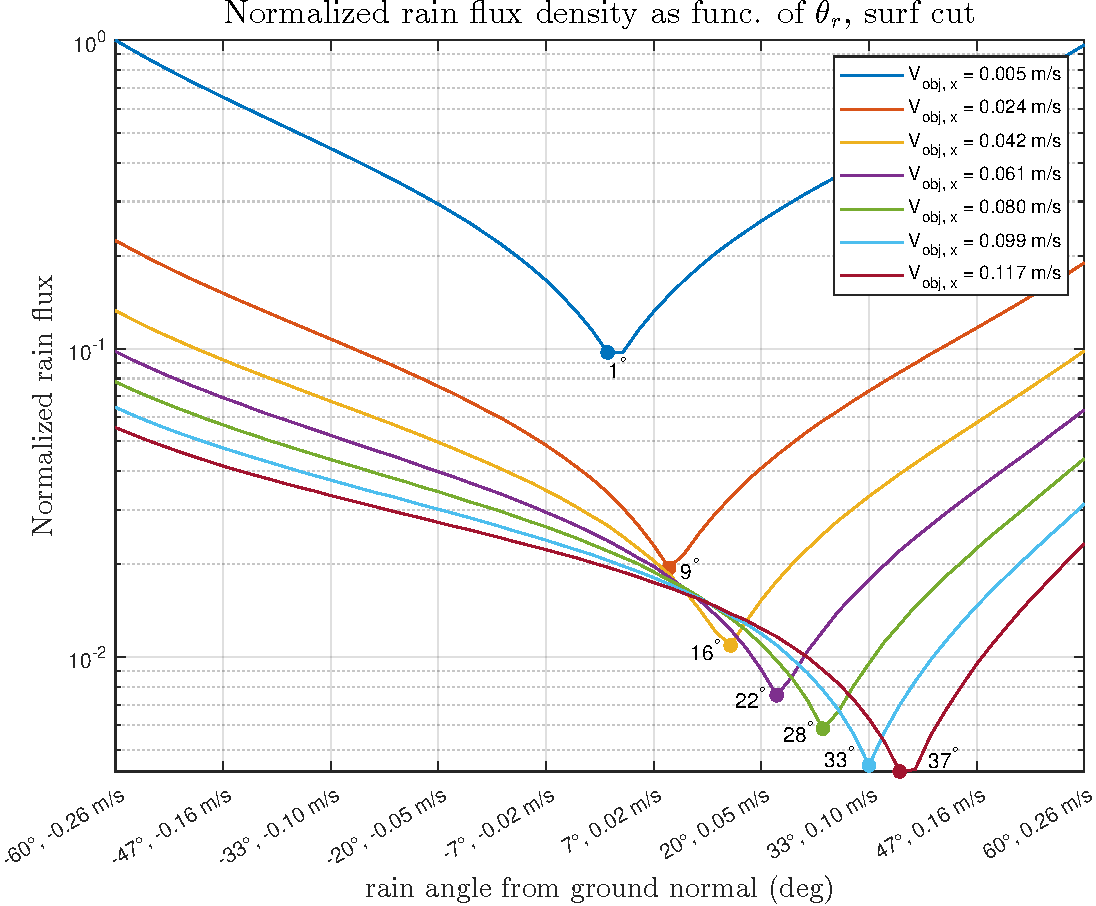
\includegraphics[width=0.625\textwidth]{images/human/rain_flux_theta_min.pdf}
                \caption{2D cut performed along the zx plane where the different curves represent the rain fluxes for different object speeds.}
            \end{figure}

            \newpage
            Additional figures for the case of the simulation of the body of a cat:
            \vspace{-10pt}
            \begin{figure}[H]
                \centering
                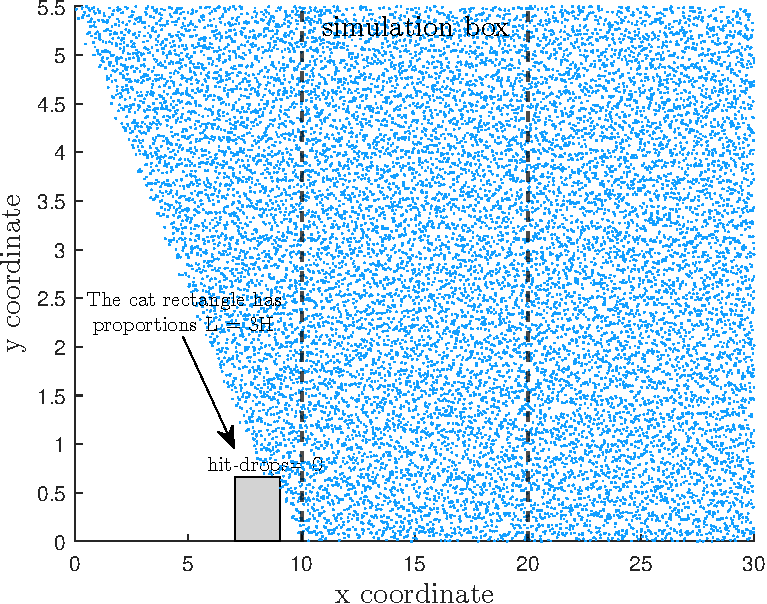
\includegraphics[width=0.625\textwidth]{images/sim_cat.pdf}
                \caption{Simulation setup in the case of the cat-shaped body. If we carefully observe the axis, the rectangle has the correct proportions (it looks taller then longer just for plotting pourposes).}
                \hspace{-5pt}
                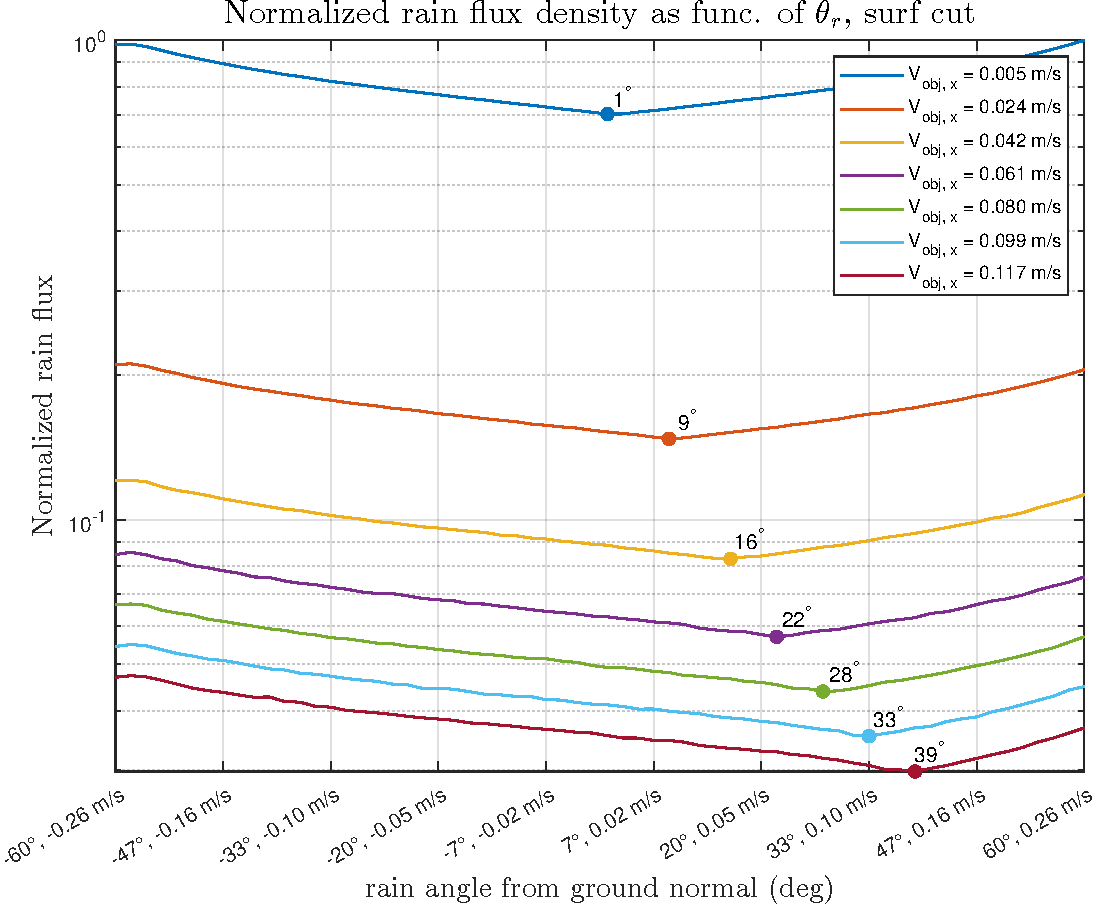
\includegraphics[width=0.625\textwidth]{images/cat/rain_flux_theta_min_cat.pdf}
                \caption{2D cut performed along the zx plane where the different curves represent the rain fluxes for different object speeds.}
            \end{figure}

            % \newpage
            % \section{MATLAB code}
            % Here is reported the MATLAB code used to create the above simulations (even if the simulations yield very good results, the code is not % optimized for speed).
            % \begin{lstlisting}[style=Matlab-editor, columns=fullflexible, escapechar=\#, numbers=left, xleftmargin=3.0ex]
            %     %% Rain simulator
            %     clc
            %     clear all;
            %     close all;
% 
            %     % --------------------------------------------------------
            %     % the rain box will be the 2D square [0, 30]^2
            %     sym.x0 = 10;
            %     sym.xe = 20;
            %     sym.y0 = 5.5;
            %     sym.ye = 0;
            %     sym.pos_toll = 1;
            %     % the rain will start from the line y = 5.5
            %     % mesh the interval [0, 30] at y = 5.5 into rain.Nr points
            %     % that will represent the number of rain drop.
            %     a = 0;
            %     b = 30;
            %     rain.Nr = 512;
            %     rain_segment = [linspace(a, b, rain.Nr)', ...
            %         sym.y0.*ones(rain.Nr, 1)];
            %     % define the rain drop y velocity rain.yVr
            %     rain.yVr = -0.150;
            %     % define the rain drop angle rain.theta_r to be the angle
            %     % that the velocity vector of each rain drops forms with
            %     % the normal vector to the ground.
            %     rain.theta_r = 0;
            %     % coefficient used to weight the effect of the added normal
            %     % random noise used to shift the newly generated rain drops
            %     rain_rand_coeff = 0.05;
            %     % parameters of the dummy human:
            %     % will be a 2D rectangle
            %     % the generic human ratio is H = 6*L
            %     human.L = 0.83;
            %     human.H = 5;
            %     human.x_pos = sym.x0 - human.L - sym.pos_toll;
            %     human.vel = 0;
            %     % --------------------------------------------------------
% 
            %     % define parameters range
            %     start_vel = 0.005;
            %     end_vel = 0.3;
            %     start_angle = pi/3;
            %     end_angle = -pi/3;
            %     % define parameters steps
            %     angle_steps = 64;
            %     human_vel_steps = 64;
            %     % compute parameters vectors
            %     vel_vect = linspace(start_vel, end_vel, human_vel_steps);
            %     angle_vect = linspace(start_angle, end_angle, angle_steps);
            %     % define the hit_drops_matrix
            %     hit_drops_matrix = zeros(angle_steps, human_vel_steps);
% 
            %     % sweep the simulation parameters rain angle and human speed
            %     for curr_vel = 1:human_vel_steps
            %         % assign current velocity
            %         human.vel = vel_vect(curr_vel);
            %         for curr_angle = 1:angle_steps
            %             % assign current angle
            %             rain.theta_r = angle_vect(curr_angle);
            %             % reset the status of the system
            %             human.x_pos = sym.x0 - human.L - sym.pos_toll;
            %             % compute the velocity vector such that it respect
            %             % the imposed y velocity and angle theta
            %             rain.Vr_vect = ... 
            %                 [rain.yVr/tan(rain.theta_r - pi/2), rain.yVr];
            %             % define a vector that will hold all the rain drops
            %             % that will be added during the storm.
            %             drops_vect = []; % n_drops x 2 matrix, ...
            %             % counter that count the number of drops that impact
            %             % with the dummy human
            %             hit_drops_cnt = 0;
            %             
            %             % start the current simulation
            %             while(1)
            %                 % update the position of all the rain drops 
            %                 % present in the drops vector using the 
            %                 % previously defined velocity vector
            %                 for drop = 1:length(drops_vect)
            %                     drops_vect(drop, :) = ...
            %                         drops_vect(drop, :) + rain.Vr_vect;
            %                 end
            %                 % generate new rain drops at y = 1 + normal noise
            %                 drops_vect = [drops_vect; rain_segment + ...
            %                     randn(rain.Nr, 2).*rain_rand_coeff];
            %                 % remove the drops outside the simulation box
            %                 drops_vect(drops_vect(:, 2) < sym.ye, :) = [];
            %                 % update the position of the dummy human
            %                 % using it's velocity value
            %                 % wait for the simulation box to be full of rain
            %                 % before starting to count drops collisions
            %                 if(nnz(drops_vect(:, 2) <= human.H) > 0)
            %                     human.x_pos = human.x_pos + human.vel;
            %                 end
            %                 % remove all the rain drops that impact the dummy
            %                 % human, the counts starts only when the human
            %                 % enters the symulation box
            %                 hit_drops = drops_vect(:, 1) > human.x_pos & ...
            %                     drops_vect(:, 1) < human.x_pos + human.L & ...
            %                     drops_vect(:, 2) < human.H;
            %                 drops_vect(hit_drops, :) = [];
            %                 if(human.x_pos > sym.x0 && human.x_pos <= sym.xe)
            %                    hit_drops_cnt = hit_drops_cnt + nnz(hit_drops);
            %                 end
            %                 % stop the simulation if the rectangle reach
            %                 % the end of the simulation box
            %                 if(human.x_pos >= sym.xe + sym.pos_toll)
            %                     break;
            %                 end
            %             end
            %             % save the number of rain drops
            %             hit_drops_matrix(curr_angle, curr_vel) = ...
            %                 hit_drops_cnt;
            %         end
            %     end
            % \end{lstlisting}

\end{document}